% L12a Farmer–Joshi market, two panels (November 5, 2026; revised the same day: panel A lost its
% repeated notes and second equation, and panel B became the position-against-signal loop of
% Farmer and Joshi's Fig. 4 instead of a state machine with three lines of text).
% A: one step of the market, with the new price feeding back into every signal.
% B: the threshold rule of a value investor. Drawn with chi_in = 2 and chi_out = -0.5, so the
% short position (-c) is entered at zeta = +2 and exited at zeta = -0.5, and the long position
% (+c) is entered at zeta = -2 and exited at zeta = +0.5. Checked against threshold_position
% (direction -1): from 0, short if zeta > chi_in, long if zeta < -chi_in; exit a short when
% zeta < chi_out, exit a long when zeta > -chi_out.
\documentclass[tikz,border=6pt]{standalone}
% Shared style for the L12a schematics (November 5, 2026), \input by each Fig-L12a-*.tex.
% Same fonts, ink, and accent colors as the L11a/L11b profit diagrams. The notebook SVG
% carries a dark palette added by theme_svg.py; every color here must be mapped there.
\usepackage[no-math]{fontspec}
\IfFontExistsTF{Arial}{\setsansfont{Arial}}{\setsansfont{TeX Gyre Heros}}
\renewcommand{\familydefault}{\sfdefault}
\usepackage{amsmath,amssymb}
\usepackage{array}
\usetikzlibrary{arrows.meta,calc,positioning,decorations.pathreplacing,shapes.geometric}

\definecolor{vnink}{HTML}{202124}
\definecolor{gdblue}{HTML}{0091FF}
\definecolor{gdred}{HTML}{E02020}
\definecolor{gdgray}{HTML}{6D7278}
\definecolor{saorange}{HTML}{F08C00}
\definecolor{boxfill}{HTML}{F1F3F4}
\definecolor{orangefill}{HTML}{FFE8C7}
\definecolor{bluefill}{HTML}{E5F3FF}
\definecolor{redfill}{HTML}{FDE8E8}
\definecolor{gridgray}{HTML}{E3E5E8}

\tikzset{
  every picture/.append style={x=1cm, y=1cm, font=\sffamily\small, text=vnink},
  flow/.style={draw=vnink, line width=0.9pt, -{Latex[length=2.4mm, width=1.7mm]}},
  feedback/.style={draw=saorange, line width=1.2pt, -{Latex[length=2.6mm, width=1.9mm]}, rounded corners=6pt},
  scorefeed/.style={draw=gdblue, line width=1.2pt, dash pattern=on 5pt off 3pt, -{Latex[length=2.6mm, width=1.9mm]}, rounded corners=6pt},
  agent/.style={draw=vnink, fill=boxfill, line width=0.8pt, rounded corners=3pt, minimum width=1.75cm, minimum height=1.05cm, align=center},
  token/.style={draw=vnink, fill=white, line width=0.7pt, minimum width=0.72cm, minimum height=0.6cm, inner sep=1pt},
  oldtoken/.style={text=gdgray, minimum width=0.72cm, minimum height=0.6cm, inner sep=1pt},
  action/.style={circle, draw=vnink, fill=white, line width=0.8pt, minimum size=0.78cm, inner sep=0pt},
  minority/.style={draw=saorange, fill=saorange, text=white, line width=0.8pt, minimum width=0.8cm, minimum height=0.66cm, font=\sffamily\small\bfseries},
  sumbox/.style={draw=vnink, fill=boxfill, line width=0.8pt, rounded corners=3pt, inner sep=5pt, align=center},
  note/.style={text=gdgray, font=\sffamily\footnotesize, align=center},
  paneltitle/.style={anchor=west, font=\sffamily\normalsize},
  state/.style={circle, draw=vnink, fill=white, line width=1.0pt, minimum size=1.25cm, inner sep=0pt, font=\sffamily\normalsize},
}


\begin{document}
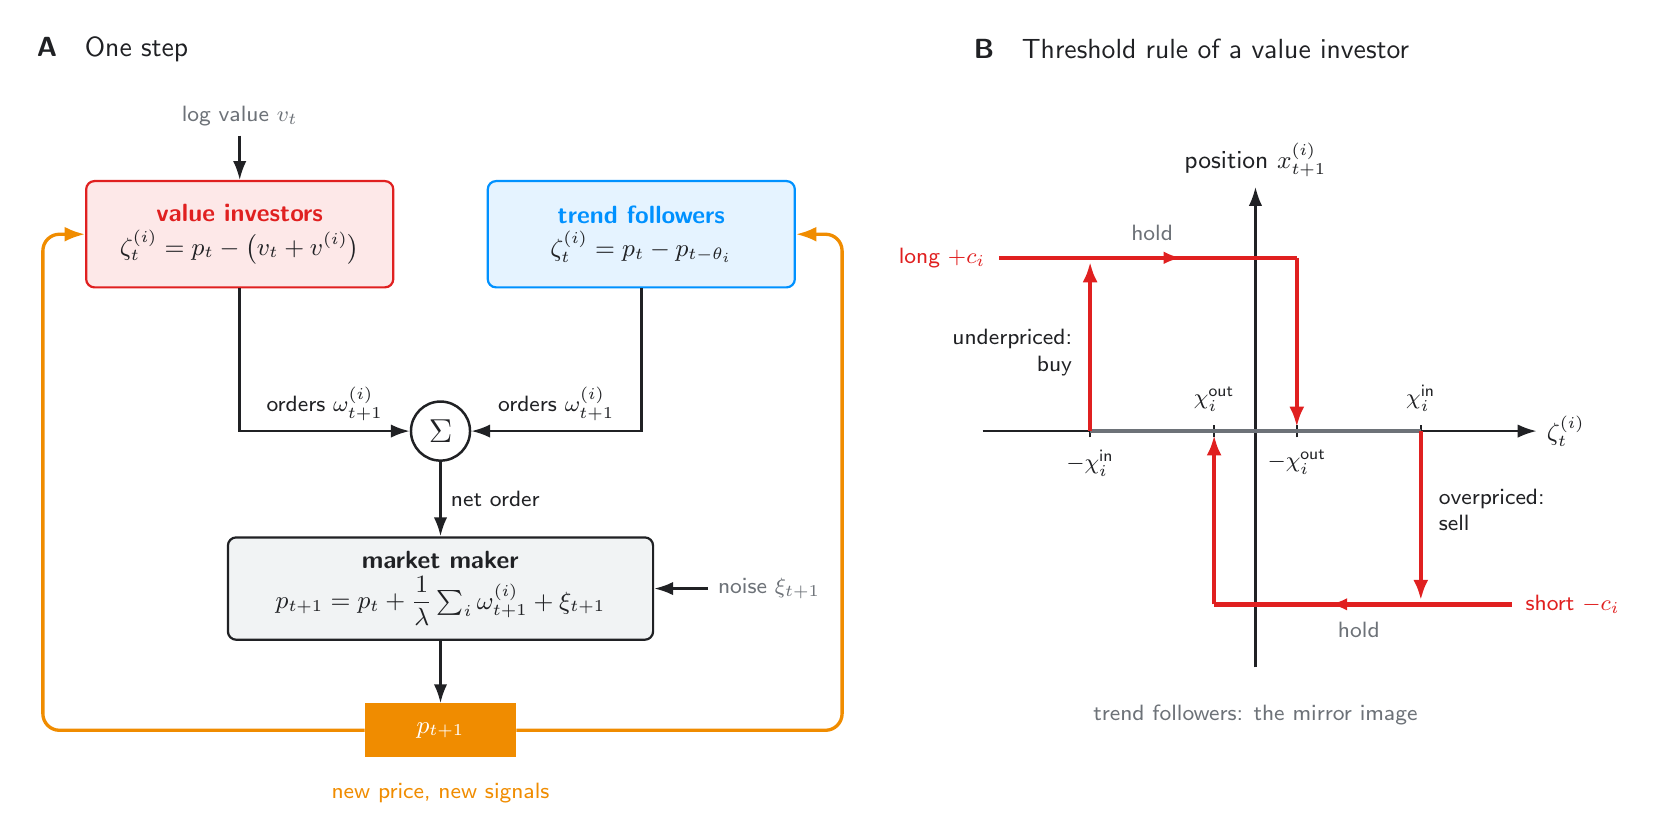
\begin{tikzpicture}
  % ================= Panel A: one step of the market =================
  \node[paneltitle] at (-0.6, 10.45) {\textbf{A}\quad One step};

  \node[note] (val) at (2.1, 9.6) {log value $v_{t}$};
  \node[agent, fill=redfill, draw=gdred, minimum width=3.9cm, minimum height=1.35cm] (vi) at (2.1, 8.1)
    {\textcolor{gdred}{\textbf{value investors}}\\[1pt]$\zeta^{(i)}_{t}=p_{t}-\bigl(v_{t}+v^{(i)}\bigr)$};
  \node[agent, fill=bluefill, draw=gdblue, minimum width=3.9cm, minimum height=1.35cm] (tf) at (7.2, 8.1)
    {\textcolor{gdblue}{\textbf{trend followers}}\\[1pt]$\zeta^{(i)}_{t}=p_{t}-p_{t-\theta_{i}}$};
  \draw[flow] (val.south) -- (vi.north);

  % orders into the net order
  \node[circle, draw=vnink, fill=white, line width=0.9pt, inner sep=1pt, minimum size=0.75cm, font=\sffamily\large] (net) at (4.65, 5.6) {$\Sigma$};
  \draw[flow] (vi.south) |- (net.west) node[pos=0.75, above, font=\sffamily\footnotesize] {orders $\omega^{(i)}_{t+1}$};
  \draw[flow] (tf.south) |- (net.east) node[pos=0.75, above, font=\sffamily\footnotesize] {orders $\omega^{(i)}_{t+1}$};

  % the market maker sets the new log price
  \node[sumbox, minimum width=5.4cm] (mm) at (4.65, 3.6)
    {\textbf{market maker}\\[2pt]$p_{t+1}=p_{t}+\dfrac{1}{\lambda}\sum_{i}\omega^{(i)}_{t+1}+\xi_{t+1}$};
  \draw[flow] (net.south) -- (mm.north) node[midway, right, font=\sffamily\footnotesize] {net order};
  \node[note, anchor=west] (noise) at (8.05, 3.6) {noise $\xi_{t+1}$};
  \draw[flow] (noise.west) -- (mm.east);

  \node[minority, minimum width=1.9cm] (price) at (4.65, 1.8) {$p_{t+1}$};
  \draw[flow] (mm.south) -- (price.north);

  % feedback: the new price changes every signal at the next step
  \draw[feedback] (price.west) -- (-0.4, 1.8) -- (-0.4, 8.1) -- (vi.west);
  \draw[feedback] (price.east) -- (9.75, 1.8) -- (9.75, 8.1) -- (tf.east);
  \node[anchor=north, text=saorange, font=\sffamily\footnotesize] at (4.65, 1.25) {new price, new signals};

  % ================= Panel B: the threshold rule as a loop =================
  \begin{scope}[xshift=15.0cm, yshift=5.6cm]
    \node[paneltitle] at (-3.7, 4.85) {\textbf{B}\quad Threshold rule of a value investor};
    % axes: signal zeta (x, 1 unit = 1.05 cm) and position (y: +c at 2.2, 0 at 0, -c at -2.2)
    \def\s{1.05}
    \draw[draw=vnink, line width=0.8pt, -{Latex[length=2.4mm, width=1.7mm]}] (-3.3*\s, 0) -- (3.4*\s, 0) node[right] {$\zeta^{(i)}_{t}$};
    \draw[draw=vnink, line width=0.8pt, -{Latex[length=2.4mm, width=1.7mm]}] (0, -3.0) -- (0, 3.1) node[above] {position $x^{(i)}_{t+1}$};
    % threshold ticks on the signal axis; each label sits on the side of the axis with no line
    \foreach \x in {-2, -0.5, 0.5, 2} {\draw[draw=vnink, line width=0.6pt] (\x*\s, -0.08) -- (\x*\s, 0.08);}
    \node[anchor=north, font=\sffamily\footnotesize] at (-2*\s, -0.12) {$-\chi^{\text{in}}_{i}$};
    \node[anchor=south, font=\sffamily\footnotesize] at (2*\s, 0.12) {$\chi^{\text{in}}_{i}$};
    \node[anchor=south, font=\sffamily\footnotesize] at (-0.5*\s, 0.12) {$\chi^{\text{out}}_{i}$};
    \node[anchor=north, font=\sffamily\footnotesize] at (0.5*\s, -0.12) {$-\chi^{\text{out}}_{i}$};

    % flat (0) between the entry thresholds
    \draw[draw=gdgray, line width=1.6pt] (-2*\s, 0) -- (2*\s, 0);
    % short branch: enter at +chi_in (down), hold, exit at chi_out (up)
    \draw[draw=gdred, line width=1.6pt, -{Latex[length=2.6mm, width=1.9mm]}] (2*\s, 0) -- (2*\s, -2.15);
    \draw[draw=gdred, line width=1.6pt] (3.1*\s, -2.2) -- (-0.5*\s, -2.2);
    \draw[draw=gdred, line width=1.6pt, -{Latex[length=2.6mm, width=1.9mm]}] (-0.5*\s, -2.2) -- (-0.5*\s, -0.05);
    \draw[draw=gdred, line width=1.2pt, -{Latex[length=2.2mm, width=1.6mm]}] (1.6*\s, -2.2) -- (0.9*\s, -2.2);
    % long branch: enter at -chi_in (up), hold, exit at -chi_out (down)
    \draw[draw=gdred, line width=1.6pt, -{Latex[length=2.6mm, width=1.9mm]}] (-2*\s, 0) -- (-2*\s, 2.15);
    \draw[draw=gdred, line width=1.6pt] (-3.1*\s, 2.2) -- (0.5*\s, 2.2);
    \draw[draw=gdred, line width=1.6pt, -{Latex[length=2.6mm, width=1.9mm]}] (0.5*\s, 2.2) -- (0.5*\s, 0.05);
    \draw[draw=gdred, line width=1.2pt, -{Latex[length=2.2mm, width=1.6mm]}] (-1.6*\s, 2.2) -- (-0.9*\s, 2.2);

    % labels: the two positions at the ends of their lines, the two entries, and the holds
    \node[anchor=east, font=\sffamily\footnotesize, text=gdred] at (-3.15*\s, 2.2) {long $+c_{i}$};
    \node[anchor=west, font=\sffamily\footnotesize, text=gdred] at (3.15*\s, -2.2) {short $-c_{i}$};
    \node[anchor=west, font=\sffamily\footnotesize, align=left] at (2.1*\s, -1.0) {overpriced:\\sell};
    \node[anchor=east, font=\sffamily\footnotesize, align=right] at (-2.1*\s, 1.0) {underpriced:\\buy};
    \node[note, anchor=south] at (-1.25*\s, 2.3) {hold};
    \node[note, anchor=north] at (1.25*\s, -2.3) {hold};
    \node[note, anchor=north] at (0, -3.35) {trend followers: the mirror image};
  \end{scope}
\end{tikzpicture}
\end{document}
